\par{``N-body methods calculate interactions between many discrete points and are characterized 
    by large numbers of in- dependent calculations within a time step, followed by all-to- all 
    communication between time steps. Our GEM code calculates the effect that all atoms have on 
    the charge at each point along the surface of a molecule, leading to O(M ∗ N ) 
    complexity where N is atoms and M is points along the surface.”\cite{dwarfs}}

\par{For this particular N Body Problem, we are computing biomelcular electrostatic 
    surface potential. The calculation of potential is done using the linearized 
    Poisson-Boltzmann model (ALPB). This is implemented in the GEM package 
    (an open-source implementation of ALPB) . The potential at any single point in space, 
    for example a vertex point on the molecular surface, is computed as a sum of contributions 
    from the individual atomic charges in the solute.}

\par{Figure \ref{nbody} and equation \ref{eq:nbody} illustrates what is being calculated and the simplified ALPB equation 
    with which the calculation is performed.}

\begin{figure}[!h]
    \centering
    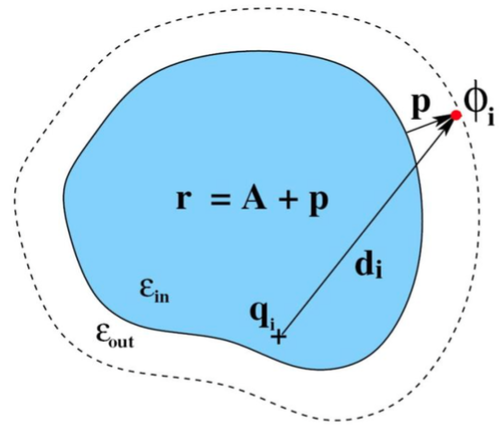
\includegraphics[width=0.5\textwidth]{figures/nbody.png}
    \caption{N-body problem.}
    \label{nbody}
\end{figure}

\begin{equation} \label{eq:nbody}
    \Phi_i^{solvent} = \frac{q_i}{\in_{out}}\frac{1}{(1+\alpha\frac{\in_{in}}{\in_{out}})}\Bigg[\frac{1+\alpha}{d_i}-\frac{\alpha(1-\frac{\in_in}{\in_out})}{r}\Bigg]
\end{equation}

\begin{itemize}
    \item $\Phi$: electrostatic potential at point of interest/observation.
    \item \emph{di}: distance from the source charge qi to the point of observation.
    \item \emph{qi}: electrostatic potential at point of interest/observation.
    \item $\alpha$: constant.
    \item  \emph{r}: distance from the point of observation to the ``centre".
    \begin{itemize}
        \item \emph{A}: effective electrostatic size of the molecule.
        \item \emph{p}: perpendicular distance of the vertex point from the surface of the molecule.
    \end{itemize}
\end{itemize}

\par{The molecular surface(solid line) separates the low dielectric interior(\in in blue region) 
    from the high dielectric solvent space, \in out.}

\par{The method of Hierarchical Charge Partitioning(HCP)(figure \ref{hpc}) is also implemented within the code, 
    to allow for greater accuracy while also restricting the computational bottlenecks. 
    HCP exploits the natural partitioning of bio molecules into constituent structural components. 
    This use of multi-scale approximations for the potential allows for speed-ups to be achieved.}

\begin{figure}[!h]
    \centering
    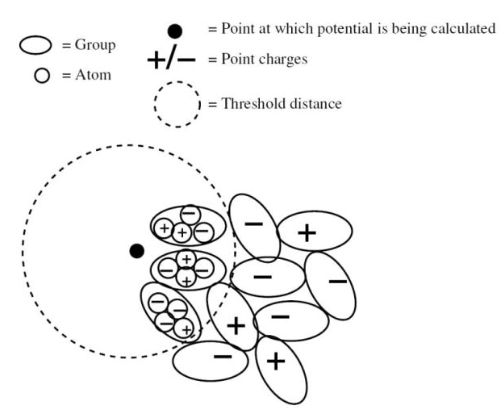
\includegraphics[width=0.5\textwidth]{figures/hpc.png}
    \caption{Hierarchical Charge Partitioning(HCP)\cite{nbody_gpu}.}
    \label{hpc}
\end{figure}

\par{The electrostatic effect of distant components is calculated from a small set of point charges. 
    Whereas, with nearby components, full sets of atomic charges are used for electrostatic interactions.}





